\chapter{Resultados e Validação} \label{ch:results}

Com o simulador finalizado, é necessária a avaliação de seus resultados para que a implementação seja validada. A apresentação e a análise de simulações são feitas neste capítulo. Com o fim de se fazer a validação numérica, os resultados são comparados com soluções analíticas ou qualitativamente avaliados.

O procedimento adotado para validação numérica da implementação considera:
\begin{alineas}
	\item a análise qualitativa da solução numérica. Por exemplo, em simulações sem forças externas, as quantidades de movimento linear e angular devem se manter constantes no sistema, e a verificação desse fato no resultado da simulação indica, nesse sentido, uma representatividade correta do fenômeno físico estudado;
	\item a comparação qualitativa com a solução analítica, se esta estiver disponível. Este item é semelhante ao anterior, mas considera ainda a solução analítica para o estudo do comportamento dos resultados numéricos; 
	\item o estudo do erro da solução numérica com relação à analítica, se esta for conhecida. O erro representa o grau de discordância entre as soluções, e valores baixos indicam a corretude do algoritmo.
\end{alineas}


O \textit{erro} de um resultado é uma medida fundamental para atestar-se a validade do método. Quanto maior o erro, menos representativa se torna a simulação. Sendo \(y\) uma solução obtida numericamente e \(\analytical{y}\) a solução exata do problema, define-se o erro de \(y\) como
\begin{equation*}
	\errorOf{y} = \abs{y - \analytical{y}}.
\end{equation*}

O erro máximo, por sua vez, é o maior erro pontual entre \(y\) e \(\analytical{y}\), isto é, é o maior elemento do conjunto imagem da função erro:
\begin{equation*}
	\maximumErrorOf{y} = \max\pqty{\Im\pqty{\errorOf{y}}}.
\end{equation*}

Para funções vetoriais \(\vec{y}\), o erro e o erro máximo são definidos equivalentemente como
\begin{gather}
	\errorOf{\vec{y}} = \norm{\vec{y} - \analytical{\vec{y}}}, \label{eq:vector_error} \\
	\maximumErrorOf{\vec{y}} = \max\pqty{\Im\pqty{\errorOf{\vec y}}}. \label{eq:maximum_vector_error}
\end{gather}

Todas as simulações foram executadas em um computador com épsilon de máquina aproximadamente igual a \(2\cdot10^{-16}\), memória \RAM{} de 16\GiB{} e processador Intel Core i7-4770 \SI{3.40}{\giga\hertz}.

Foram escolhidos quatro problemas a serem apresentados e estudados: o problema do lançamento oblíquo, em que uma partícula é lançada no espaço sujeita unicamente à ação da gravidade; o problema da esfera quicando, em que uma partícula liberada no espaço em repouso é atraída, pela gravidade, em direção ao chão, colidindo com ele; a colisão com rotação, em que duas esferas se chocam, sendo que uma delas possui velocidade angular não nula; e o problema da queda com arrasto, em que uma partícula é solta no espaço e cai em decorrência da ação da gravidade, sofrendo, ao longo de sua trajetória, a resistência do ar.

\section{Lançamento Oblíquo} \label{sec:free_fall}

O lançamento oblíquo é um dos problemas clássicos de física básica. Considera-se uma partícula de massa \(\mass\) sujeita unicamente à ação de um campo gravitacional constante cuja aceleração da gravidade é \(\gravity\). Nessas condições, as equações de movimento para a partícula se tornam, simplesmente,
\begin{gather}
	\acceleration = \gravity, \label{eq:free_fall_translation}\\
	\angularAcceleration = \nullVector \label{eq:free_fall_rotation}.
\end{gather}

O instante inicial da simulação é definido como \(\initialInstant=0\), e o instante final é um valor arbitrário \(\finalInstant\). A posição, a velocidade e a velocidade angular da partícula no instante inicial assumem, respectivamente, os valores \(\initial{\position}\), \(\initial{\velocity}\) e \(\initial{\angularVelocity}\). Com isso, as equações \eqref{eq:free_fall_translation} e \eqref{eq:free_fall_rotation} podem ser resolvidas por integração simples:
\begin{gather*}
	\acceleration\pqty{t} = \gravity, \\
	\velocity\pqty{t} = \initial{\velocity} + \int_{\initialInstant}^{t} \acceleration\pqty{\tau} \dd{\tau} = \initial{\velocity} + \gravity\cdot t, \\
	\position\pqty{t} = \initial{\position} + \int_{\initialInstant}^{t} \velocity\pqty{\tau} \dd{\tau} = \initial{\position} + \initial{\velocity}\cdot t + \gravity\cdot \dfrac{t^2}{2}, \\
	\angularVelocity\pqty{t} = \initial{\angularVelocity} + \int_{\initialInstant}^{t} \nullVector \dd{\tau} = \initial{\angularVelocity}.
\end{gather*}

Por simplicidade, considera-se que o movimento ocorra apenas no plano \(\xAxis\yAxis\), que a gravidade atue no sentido negativo do eixo \(\yAxis\), isto é, \(\gravity = -\gravityScalar\cdot\yUnit\) com \(\gravityScalar>0\), e que a partícula não possua rotação, como representado na figura \ref{fig:free_fall}. Nessa situação, a posição em \(\yAxis\) da partícula é chamada de altura.

\begin{figure}[h]
	\caption{O problema do lançamento oblíquo}
	% \vspace{-0.5cm}
	\centering
		\alert{Colocar imagem representando o problema do lançamento oblíquo}
		% 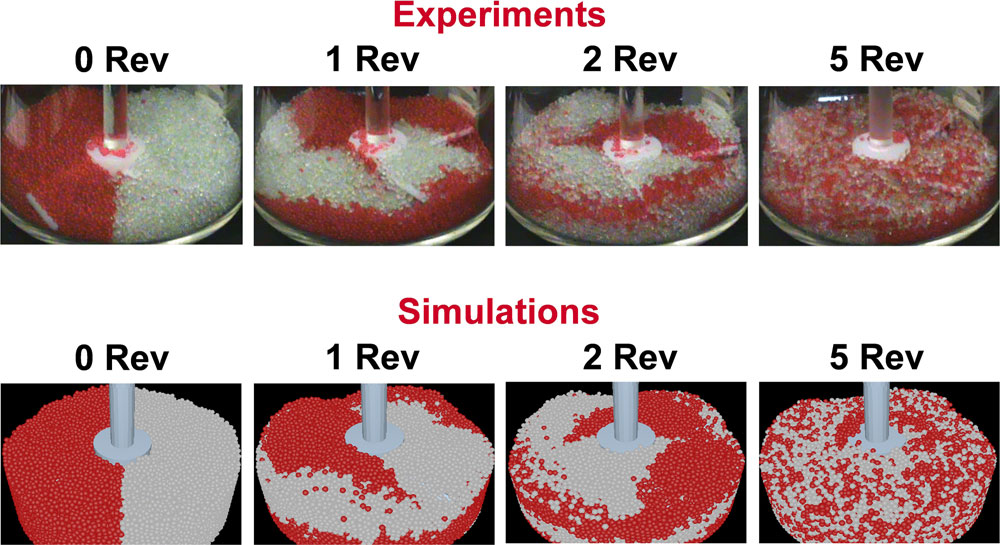
\includegraphics[width=0.65\textwidth]{images/drug_production.png}
	% {\centerline{\includegraphics[scale=#2]{#1}}}
	% \vspace{-0.2cm}
	\label{fig:free_fall}
	\source{\alert{Citar fonte}}
	% \vspace{-1cm}
\end{figure}

Com isso, escrevendo \(\position = \explicitVectorCoordinates{\positionScalar}\), \(\velocity = \explicitVectorCoordinates{\velocityScalar}\) e \(\acceleration = \explicitVectorCoordinates{\accelerationScalar}\), é obtida a solução como apresentada na tabela \ref{table:free_fall_solution}.

\begin{table}[h]
	\caption{Solução do problema do lançamento oblíquo}
	\label{table:free_fall_solution}

	\begin{equation*}
		\arraycolsep=1.5\arraycolsep
		\def\arraystretch{1.5}
		\begin{array}{lcc}
	\hline
		& \text{Direção } \xAxis 
		& \text{Direção } \yAxis \\
	\text{Posição} 
		& \positionx = \initial{\positionx} + \initial{\velocityx}\cdot \Dt
		& \positiony = \initial{\positiony} + \initial{\velocityy}\cdot \Dt - \dfrac{\gravityScalar\Dt^2}{2} \\
	\text{Velocidade} 
		& \velocityx = \initial{\velocityx}
		& \velocityy = \initial{\velocityy} - \gravityScalar\cdot \Dt \\
	\text{Aceleração} 
		& \accelerationx = 0
		& \accelerationy = - \gravityScalar \\
	\hline	
		\end{array}
	\end{equation*}
	\sourceMe
\end{table}

Embora seja conceitualmente simples e de fácil resolução, o problema do lançamento oblíquo permite:
\begin{itemize}
\item A validação numérica da implementação do algoritmo de Gear em simulações sem colisões, mas com a atuação de forças de campo. Em cada instante, as coordenadas da partícula são previstas e, em seguida, corrigidas a partir do valor da força da gravidade. A proximidade da resposta numericamente calculada com a solução analítica evidencia o bom funcionamento do algoritmo.
\item A obtenção da evolução do erro com o tempo de simulação. Não só existe um erro associado ao método como esse erro se acumula com o tempo.
\end{itemize}

A fim de se compararem os resultados numéricos com a solução analítica, foram arbitrados aos parâmetros do problema os valores dispostos na tabela \ref{tab:free_fall_case_parameters}.

\begin{table}[h]
\centering
\caption{Parâmetros para o \alert{estudo de caso} do problema de lançamento oblíquo.}
\label{tab:free_fall_case_parameters}
\begin{parametersdesc}
	\item{Massa da partícula}{\mass = 1}{\si\kilogram}
	\item{Raio da partícula}{\radius = 3}{\si\centi\metre}
	\item{Posição inicial}{\explicitVector{\initial{\positionx}}{\initial{\positiony}}{\initial{\positionz}} = \explicitNumericVector{0}{0}{0}}{\si{\metre}}
	\item{Velocidade inicial}{\explicitVector{\initial{\velocityx}}{\initial{\velocityy}}{\initial{\velocityz}} = \explicitNumericVector{20}{10}{0}}{\si[per-mode=symbol]{\metre\per\second}}
	\item{Aceleração inicial}{\explicitVector{\initial{\accelerationx}}{\initial{\accelerationy}}{\initial{\accelerationz}} = \explicitNumericVector{0}{-9,81}{0}}{\si[per-mode=symbol]{\metre\per\square\second}}
	\item{Instante final}{\finalInstant = 3}{\si\second} 
	\item{Ordem de extrapolação}{\taylorOrder = 7}{\emptyUnit}
	\item{Gravidade}{\gravityScalar = 9,81}{\si[per-mode=symbol]{\metre\per\square\second}}
	\item{Passo de tempo}{\Dt = 10^{-3}}{\si\second}
\end{parametersdesc}
\sourceMe 
\end{table}

Muito embora se trate de um problema bidimensional sem rotação, o simulador utiliza a formulação tridimensional e considera a evolução da velocidade angular da partícula.

\begin{figure}[h]
	\caption{Solução para a altura da partícula no problema de lançamento oblíquo\protect\footnotemark.}
	% \vspace{-0.5cm}
	\centering
		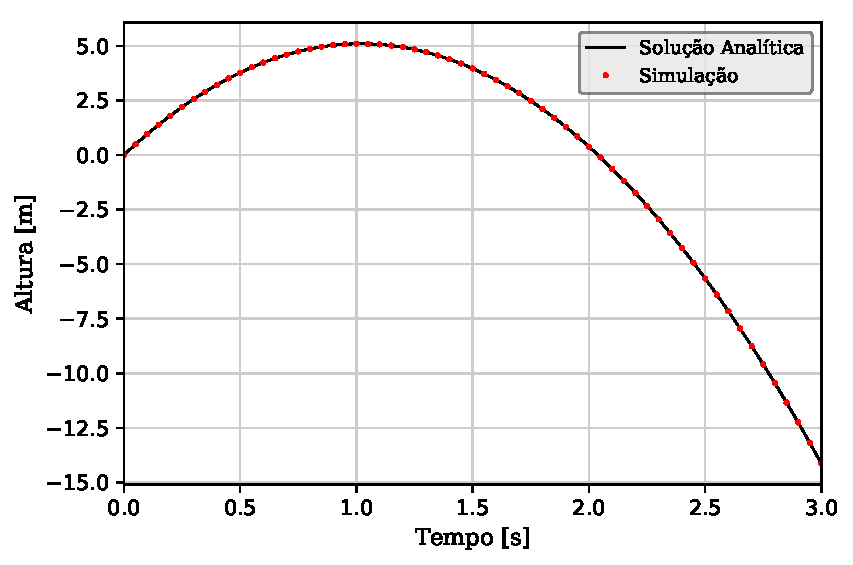
\includegraphics[scale=1]{images/falling_sphere/correct_initial_acceleration/y_position.pdf}
		% 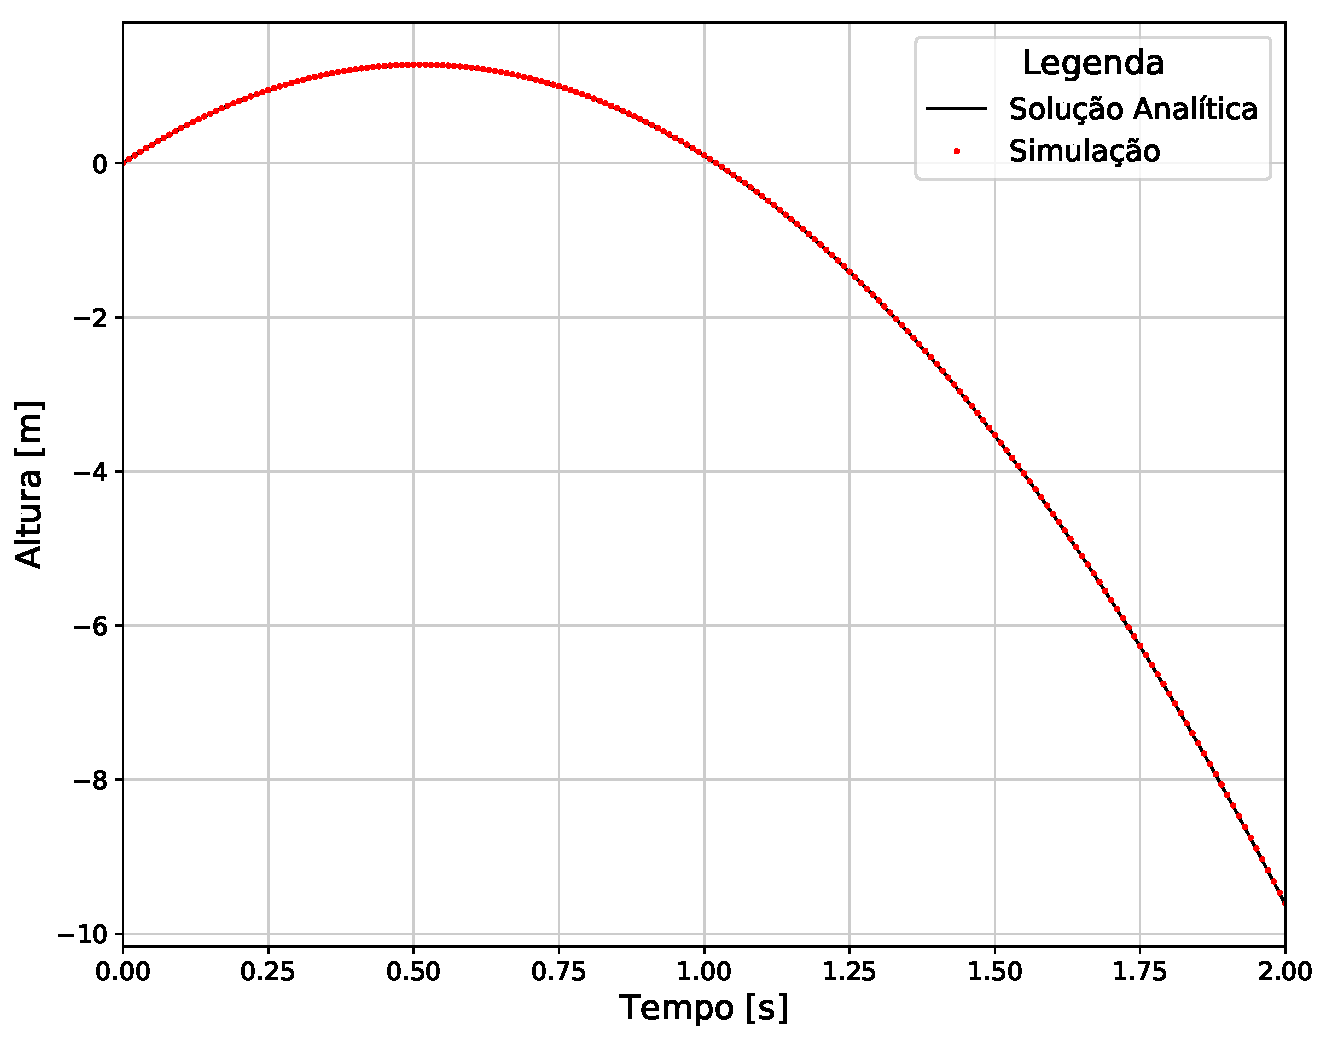
\includegraphics[width=\normalresultsfigwidth]{images/falling_sphere/y_position.pdf}
	% {\centerline{\includegraphics[scale=#2]{#1}}}
	% \vspace{-0.2cm}
	\label{fig:falling_sphere_y_position}
	\sourceMe
	% \vspace{-1cm}
\end{figure}

\footnotetext{Para melhor visualização dos resultados, é apresentado um ponto a cada dez passos de tempo.}

\begin{figure}[h]
	\caption[Solução do problema de lançamento oblíquo para a posição horizontal, a velocidade horizontal, a velocidade vertical e a aceleração vertical da partícula]{Solução do problema de lançamento oblíquo para (\subref{subfig:x_position}) a posição horizontal, (\subref{subfig:x_velocity}) a velocidade horizontal, (\subref{subfig:y_velocity}) a velocidade vertical e (\subref{subfig:y_acceleration}) a aceleração vertical da partícula}
	% \vspace{-0.5cm}
	\centering
	\captionsetup[subfloat]{labelfont=bf}
	\subfloat{
		\centering
		\begin{subfigure}[t]{\smallresultsfigwidth}
			\centering
			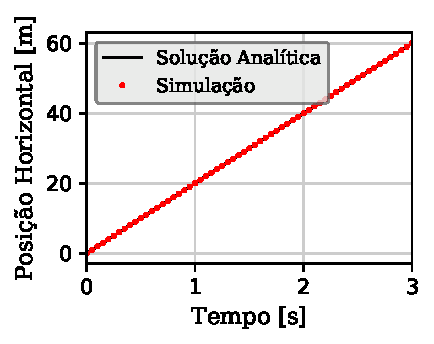
\includegraphics[scale=1]{images/falling_sphere/correct_initial_acceleration/x_position.pdf}
			\caption{}
			\label{subfig:x_position}
		\end{subfigure}
		\begin{subfigure}[t]{\smallresultsfigwidth}
			\centering
			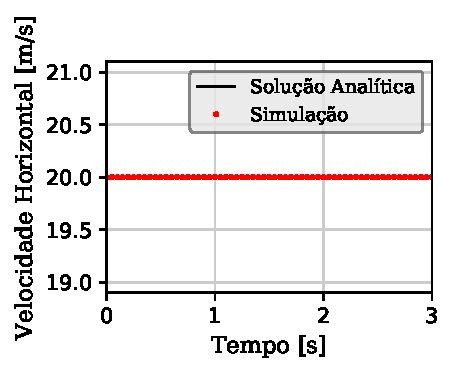
\includegraphics[scale=1]{images/falling_sphere/correct_initial_acceleration/x_velocity.pdf}
			\caption{}
			\label{subfig:x_velocity}
		\end{subfigure}
		\begin{subfigure}[t]{\smallresultsfigwidth}
			\centering
			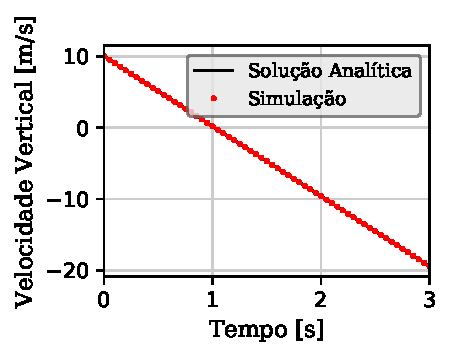
\includegraphics[scale=1]{images/falling_sphere/correct_initial_acceleration/y_velocity.pdf}
			\caption{}
			\label{subfig:y_velocity}
		\end{subfigure}
		\begin{subfigure}[t]{\smallresultsfigwidth}
			\centering
			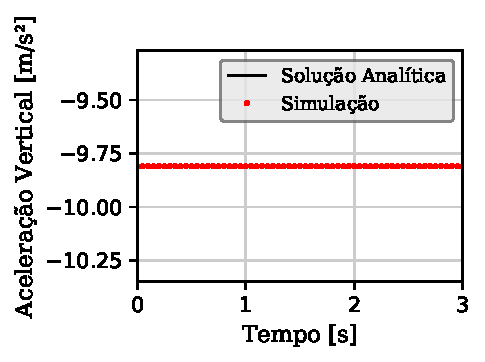
\includegraphics[scale=1]{images/falling_sphere/correct_initial_acceleration/y_acceleration.pdf}
			\caption{}
			\label{subfig:y_acceleration}
		\end{subfigure}
	}
	% {\centerline{\includegraphics[scale=#2]{#1}}}
	% \vspace{-0.2cm}
	\label{fig:falling_sphere_other}
	\sourceMe
	% \vspace{-1cm}
\end{figure}

Com esses parâmetros, foi calculada a trajetória da partícula através do simulador e da solução analítica. Na \cref{fig:falling_sphere_y_position} estão expostas as soluções para a altura da partícula, isto é, para a componente de posição \(\yComponent\positionScalar\). Observa-se nessa figura que os resultados obtidos pelo simulador se aproximam bastante da solução analítica das equações.

Outras variáveis, como a posição horizontal, as velocidades horizontal e vertical e a aceleração vertical estão apresentados na \cref{fig:falling_sphere_other}.

\begin{figure}[h]
	\caption[Erro da simulação com relação à solução numérica para a posição e da partícula do problema do lançamento oblíquo]{Erro da simulação com relação à solução numérica para (\subref{subfig:position_error}) a posição e (\subref{subfig:velocity_error}) da partícula do problema do lançamento oblíquo}
	% \vspace{-0.5cm}
	\centering
	\captionsetup[subfloat]{labelfont=bf}
	\subfloat{
		\centering
		\begin{subfigure}[t]{\smallresultsfigwidth}
			\centering
			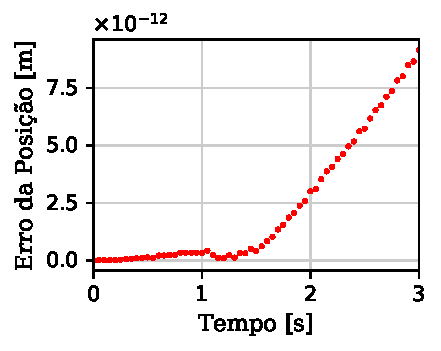
\includegraphics[scale=1]{images/falling_sphere/correct_initial_acceleration/position_error.pdf}
			\caption{}
			\label{subfig:position_error}
		\end{subfigure}
		\begin{subfigure}[t]{\smallresultsfigwidth}
			\centering
			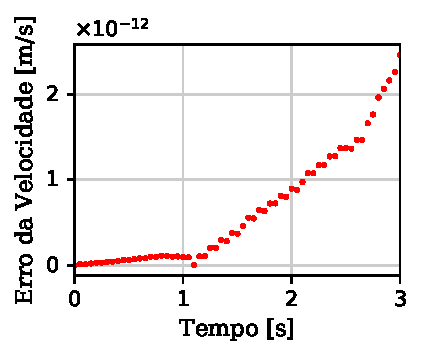
\includegraphics[scale=1]{images/falling_sphere/correct_initial_acceleration/velocity_error.pdf}
			\caption{}
			\label{subfig:velocity_error}
		\end{subfigure}
	}
	% {\centerline{\includegraphics[scale=#2]{#1}}}
	% \vspace{-0.2cm}
	\label{fig:falling_sphere_error}
	\sourceMe
	% \vspace{-1cm}
\end{figure}

Por sua vez, o erro da posição e o erro da velocidade, como funções do tempo, são apresentados na \cref{fig:falling_sphere_error}. Esses erros são calculados de acordo com a equação \eqref{eq:vector_error}. Observa-se nessa \namecref{fig:falling_sphere_error} que o erro da posição se mantém inferior a \SI{0,01}{\nano\meter} durante toda a simulação, evidenciando a exatidão do método. Além disso, é possível inferir que o erro se acumula com o avanço da simulação.

O arquivo em formato \JSON{} utilizado para essa simulação é apresentado no \cref{app:code_listings}.

\section{Esfera Quicando}

Como extensão do problema de queda livre, o problema da esfera quicando inclui, além da gravidade, a colisão entre uma esfera e uma parede plana. Supõe-se uma partícula \(\particle\) esférica de raio \(\radius\) e massa \(\mass\) que, no instante inicial \(\initialInstant=0\), é liberada no espaço, em repouso, na posição \(\initial{\position} = \explicitVector{0}{\initial{\yComponent{\positionScalar}}}{0}\).

A partícula está sujeita a um campo gravitacional constante cuja aceleração da gravidade é \(\gravity = -\gravityScalar\cdot\yUnit\) com \(\gravityScalar>0\). Nessa situação, a componente \(\yComponent{\positionScalar}\) denota a altura da partícula.

Além disso, considera-se um elemento \(\element\) identificado com o plano \(\xAxis\zAxis\) representando o chão. Sendo um plano fixo, esse elemento é completamente determinado ao se fornecerem um ponto e um versor normal a ele. Para o plano \(\xAxis\zAxis\), podem ser adotados a origem \(\originPoint\) do sistema como ponto pertencente ao plano e o versor normal \(\planeNormalVersor = \explicitVector{0}{1}{0}\).

Esse problema pode ser representado como na figura \ref{fig:bouncing_sphere}.

\begin{figure}[h]
	\caption{O problema da esfera quicando}
	% \vspace{-0.5cm}
	\centering
		\alert{Colocar imagem representando o problema da esfera quicando}
		% 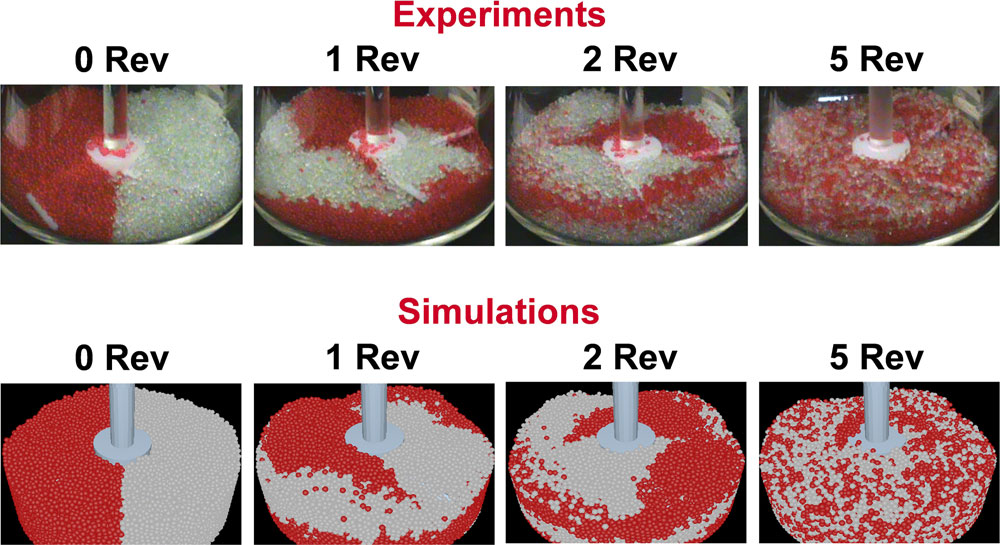
\includegraphics[width=0.65\textwidth]{images/drug_production.png}
	% {\centerline{\includegraphics[scale=#2]{#1}}}
	% \vspace{-0.2cm}
	\label{fig:bouncing_sphere}
	\source{\alert{Citar fonte}}
	% \vspace{-1cm}
\end{figure}

Além de servir como mais um caso para a validação do código, o problema da esfera quicando possibilita a comparação entre o coeficiente de restituição calculado a partir dos resultados da simulação e o coeficiente calculado analiticamente a partir do modelo de força escolhido.

A configuração do problema implica que a velocidade da esfera relativa ao plano é a sua própria velocidade vertical, já que o plano não se movimenta. Como consequência das equações \eqref{eq:antisymmetry_relative_velocity} e \eqref{eq:sphere_plane_relative_velocity}, essa velocidade é a própria velocidade da partícula.

Com isso, sendo \(\coefficientOfRestitution\) o coeficiente de restituição associado ao modelo de força de colisão escolhido, é possível mostrar que
\begin{equation*}
	\coefficientOfRestitution = - \dfrac{\afterCollision{\yComponent{\velocityScalar}} + \gravityScalar\cdot\collisionDuration}{\beforeCollision{\yComponent{\velocityScalar}}},
\end{equation*}
sendo \(\afterCollision{\yComponent{\velocityScalar}}\) a velocidade da partícula \(\particle\) após a colisão com o chão, e \(\collisionDuration\), o tempo em que os corpos permanecem em contato. O termo \(\gravityScalar\cdot\collisionDuration\) é uma compensação feita pelo fato de que, no problema em questão, a gravidade contribui para a variação da velocidade das partículas, o que não é considerado no cálculo analítico do coeficiente de restituição.

\alert{Análises a se fazerem: comparação entre o coeficiente de restituição calculado e o analítico.}

\subsection{\alert{Estudo de Caso}}

Para o estudo do problema da esfera quicando, foram considerados os parâmetros de simulação expostos na tabela \ref{tab:bouncing_sphere_case_parameters}.

\begin{table}[h]
\centering
\caption{Parâmetros para o \alert{estudo de caso} do problema da esfera quicando.}
\label{tab:bouncing_sphere_case_parameters}
\begin{parametersdesc}
	\item{Modelo de força}{Amortecedor linear \alert{com correção ou não?}}{\emptyUnit}
	\item{Gravidade}{\gravityScalar = 9,81}{\si[per-mode=symbol]{\metre\per\square\second}}
	\item{Massa da partícula}{\mass = 1}{\si\kilogram}
	\item{Raio da partícula}{\radius = 3}{\si\centi\metre}
	\item{Altura inicial}{\initial{\positiony} = 1}{\si{\metre}}
	\item{Velocidade inicial}{\explicitVector{\initial{\velocityx}}{\initial{\velocityy}}{\initial{\velocityz}} = \explicitVector{0}{0}{0}}{\si[per-mode=symbol]{\metre\per\second}}
	\item{Aceleração inicial}{\explicitVector{\initial{\accelerationx}}{\initial{\accelerationy}}{\initial{\accelerationz}} = \explicitNumericVector{0}{0}{0}}{\si[per-mode=symbol]{\metre\per\square\second}}
	\item{Instante final}{\finalInstant = 3}{\si\second} 
	\item{Ordem de extrapolação}{\taylorOrder = 7}{\emptyUnit}
	\item{Passo de tempo}{\Dt = 10^{-3}}{\si\second}
\end{parametersdesc}
\sourceMe 
\end{table}

\section{Colisão com Rotação}

\alert{Análises a se fazerem: Conservação da quantidade de movimento linear e da quantidade de movimento angular. Conservação da energia quando os termos dissipativos são nulos. Energia perdida no caso contrário.}

\section{Queda com Arrasto}

\alert{...}

Segundo \citeonline[p. 392]{bib:fox},
\begin{equation*}
	\dragForce = \dragCoefficient\ \frac{1}{2}\density\ \projectedArea\ \norm{\velocity} \velocity
\end{equation*}
\alert{Erro! não podemos dividir por vetor...}